\section{Implementation}
\label{sec:implementation}

Our Python-based JPEG-like compression system is designed with modularity and experimentation in mind. It mirrors key stages of the classical JPEG pipeline while allowing for customized configurations through YAML files. In this section, we describe the architecture and underlying algorithms for each major component of our system, which include preprocessing, block-based Discrete Cosine Transform, quantization, entropy encoding, and full decompression support.

\subsection{Overall Compression Pipeline Structure}
The compression process consists of the following sequential stages:
\begin{enumerate}
    \item \textbf{Image Initialization}: Loading the configuration, the image, and ensuring the right format of the latter
    \item \textbf{Color Conversion}: Transforming the RGB image into YCbCr
    \item \textbf{Chrominance Downsampling}: Downsampling the two chrominance channels depending on configuration
    \item \textbf{Block Processing}: Channels get split into blocks, to each of them the following is applied
    \begin{enumerate}
    	\item \textbf{Discrete Cosine Transform (DCT)}: Transforming spatial pixel values to frequency domain.
		\item \textbf{Quantization}: Reducing frequency resolution based on configurable quantization tables.
    \end{enumerate}
    \item \textbf{Entropy Encoding}: Lossless entropy-encoding of block coefficients to compress data
        \begin{enumerate}
    	\item \textbf{Zigzagging}: Flattening the blocks
    	\item \textbf{Delta Encoding}: Take the differences of DC coefficients
    	\item \textbf{Run-Length Encoding}: Shortening AC component Array 
    	\item \textbf{Huffman Encoding}: Finding and encoding data with minimum length code 
    \end{enumerate}
    \item \textbf{File Encoding}: Encodes data and header into binary file, collects metrics
\end{enumerate}
\noindent
The decompression process reverses each of these steps.
\noindent
Each of the above steps is parameterized through YAML configuration files. Users can adjust quality settings, block sizes, quantization levels, and downsampling rates to generate different compression schemes.

\subsection{Image initialization}
\label{sec:initialization}
First, the configuration, if one has been provided either during initialization or calling of the image compressor object, is loaded, overwriting the default parameters.
Then the image gets loaded using the \texttt{scikit-image} library, unless it is a raw image file like CR2 in which case the loading is handled by using the \texttt{rawpy} wrapper for the \texttt{LibRaw} library.

Following the initial loading, all but the RGB channels get removed, since JPEG compression, with the exception of JPEG XL does not handle those. Furthermore, in case the channels have values outside of the 8 bit range (0 to 255), those get normalized and converted to unsigned integer 8 bit values per channel.

Thus, if we let  \(\bm{x} = (x,y)^T\) denote pixel coordinates, 
where $x \in \{0, \dots, w-1\}$ and $y \in \{0, \dots, h-1\}$, we now have the following RGB image $I$ which maps $\bm{x}$ to intensity values:
\[
I_{\text{RGB}}(\bm{x}) = \big( R(\bm{x}),\, G(\bm{x}),\, B(\bm{x}) \big) \in \{0, \dots, 255\}^3.
\]
Here each element of \( I(x, y) = (R(x,y), G(x,y), B(x,y)) \) contains three 8-bit unsigned integers, which are the RGB channels and are forwarded to color conversion.

\subsection{Color Conversion}
\label{sec:color}
JPEG's lossy compression relies to a good extent on downsampling the chrominance of an image. This is done as human vision is less sensitive to color variations than to brightness variations, and will therefore not perceive the downsampling of colors as much, while saving a lot of space.
To enable the chrominance downsampling, however, we first need to differentiate the luminance and chrominance parts of the images. This is done by converting RGB images to the YCbCr color space:
\begin{equation}
I_{\text{RGB}}(\bm{x}) = \begin{bmatrix} Y(\bm{x}) \\ Cb(\bm{x}) \\ Cr(\bm{x}) \end{bmatrix}
\end{equation}
\begin{equation}
= \begin{bmatrix} 0.299 & 0.587 & 0.114 \\ -0.1687 & -0.3313 & 0.5 \\ 0.5 & -0.4187 & -0.0813 \end{bmatrix} \begin{bmatrix} R(\bm{x}) \\ G(\bm{x}) \\ B(\bm{x}) \end{bmatrix} + \begin{bmatrix} 0 \\ 128 \\ 128 \end{bmatrix}
\end{equation}

\subsection{Downsampling}
To downsample the resulting YCbCr image, the chrominance channels are processed as follows depending on a downsampling factor  $d \in \mathbb{N}^+$. 
If \(d > 1\), a running average is put into place for each of the two chrominance channels, only taking every \(d\)-th pixel in such a way that the dimensions of the resulting \(\tilde{Cb}\) and \(\tilde{Cr}\) are as follows. 
\[
(h_c, w_c) = \left( \left\lceil \frac{h}{d} \right\rceil, \left\lceil \frac{w}{d} \right\rceil \right)
\]
These are then rounded to integers and put in a python list together with the unchanged Y channel. It obviously doesn't make sense anymore to represent the image as a regular array, instead they are being treated as 3 arrays in a python list.

If \(d = 1\), or in other words downsampling is not to be applied, it will just return the YCbCr channels in a list, to save computation time instead of doing an identity operation.
It is important to note that this is different than how downsampling is executed in the JPEG standard. 
With JPEG compression, the downsampling is performed by keeping individual pixels values in a pattern.
This is done with speed, rather than accuracy or quality in mind. 
For small downsample factors, keeping individual pixel values and averaging nearby pixels does essentially the same thing, but we are also interested in the compression behavior when downsample factors become very large, at which point there will be a noticeable difference between individual pixels and average pixel downsampling approaches.

\subsection{Block Processing}
To go from here, each channel is divided into usually square non-overlapping blocks using the block size parameter \(b \in \mathbb{N}^+\) (e.g. 8 is used in standard JPEG, ours is configurable). In cases where \(h \mod b \neq 0\) or \(w \mod b \neq 0\) for either the regular or the chrominance dimensions, the blocks will not be square, which is something that needs to be accounted for later. 

\subsubsection{Discrete Cosine Transform}
First, the unsigned 8 bit integer blocks are converted to signed 16 bit integers, while getting centered to zero by subtracting 128.

Then, an orthonormal type II 2D Discrete Cosine Transform (DCT), which is a real-valued offshoot of the Discrete Fourier Transform (DFT), is applied to each block using the following formula:

\begin{align}
  &F(u, v) = \frac{2}{\sqrt{N \, M}} C(u)C(v) \\ \sum_{x=0}^{N-1} \sum_{y=0}^{M-1} f(x,y)
  &\cos\left( \frac{(2x+1)u\pi}{2N} \right) \cdot \cos\left( \frac{(2y+1)v\pi}{2M} \right)
\end{align}

where $C(k) = \frac{1}{\sqrt{2}}$ if $k = 0$ and $C(k) = 1$ otherwise. The two axes (x and y) have their own respective sum indicies because our compression pipeline tolerates images with lengths and widths in pixels not divisible by the block size. This leaves results in some of the blocks being rectangular, so the axes need to be dealt with separately. Because the block represents only a small portion of the image, which usually includes very little varriation across the block, most of the image energy is usually concentrated into the upper-left lower-frequency corner of the DCT block.

Our implementation hereby leverages \texttt{scipy.fftpack.dct} for speed and numerical accuracy.

\subsubsection{Quantization}
Quantization now discards high-frequency DCT coefficients in each block, by dividing element-wise with a previously configured quantization matrix $Q \in \mathbb{N}^{b\times b}$. This is done to reduce the amount of less information carrying, nonzero components which makes Run-Length-Encoding later on much more effective. It should be noted that different quantization matrices are used for luminance and chrominance, with the latter usually receiving harsher quantization. Each coefficient $F(u,v)$ is divided by a quantization matrix $Q(u,v)$ and rounded:

 %Skipping of higher-frequency basis functions often leads to so-called blocking artifacts, but also ringing is observed particularly in case of image edge structures.

\begin{equation}
F_Q(u,v) = \left\lfloor \frac{F(u,v)}{Q(u,v)} + 0.5 \right\rfloor
\end{equation}

If the block dimensions do not match the dimensions of the quantization matrix, because of it being part of the lower or right border of the image with the image dimension not being divisible with \(b\), the block gets padded with zeros until it reaches them.

The highest-frequency component is principally set to zero to avoid issues with the zigzagging algorithm later on.

\begin{equation}
	F_Q(b-1,b-1) = 0
\end{equation}

The JPEG quantization matrix values are highly tuned and optimized across a range of quality factor for 8x8 blocks.
However, because one of the goals of this projects is to understand compression characteristics across a range of bloc sizes, we need to be able to generate quantization parameters that quantize a similar portion of the matrix for a range of block sizes. 
Because of this, we implemented two different functions that generate quantization matrix values from a small set of parameters.
\begin{itemize}
    \item \textbf{Baseline JPEG-style}: A scaled standard luminance matrix.
    \item \textbf{Quarter-Gauss-Distribution}: Tighter control on high frequencies.
    \item \textbf{LN-Norm}: Control over mid-range frequencies and their quantization level relative to high and low frequency component quantization.
    \item \textbf{Custom sweep}: Users can specify arbitrary YAML matrices.
\end{itemize}

\subsubsection{Quarter-Gauss-Distribution Quantization}

The so called "Quarter Gauss" quantization matrix function generates a quantization matrix of size NxN, using three parameters: The block size ($N$), the max quantization value ($A$), and the standard deviation ($\sigma$).

Let $d_{ab}$ be the L2 norm distance of a matrix entry $M_{ab}$from matrix element $M_{NN}$.

Then each element of the quantization matrix can be generated as shown in figure \ref{fig:gaussian_quant}

\begin{figure}
	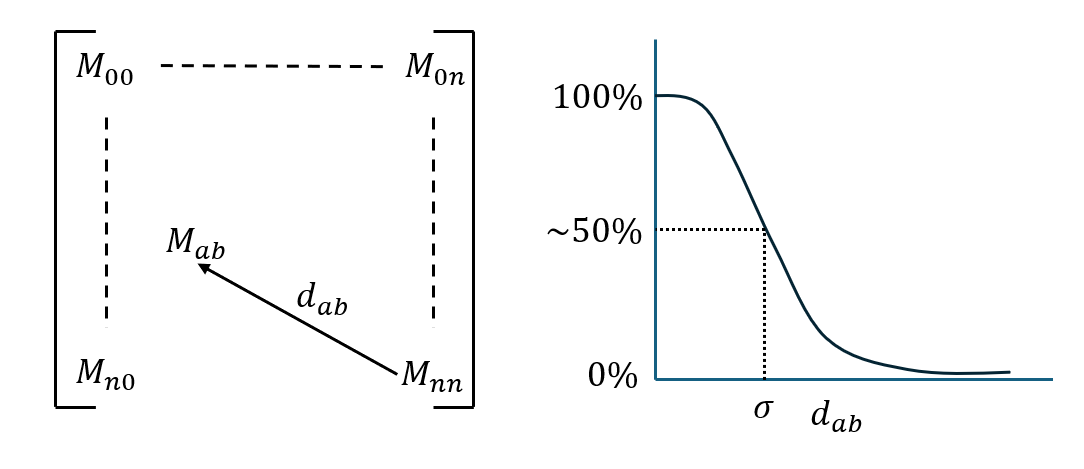
\includegraphics[width=0.5\textwidth]{assets/Quarter Gauss Quantization.png}
	\caption{Visual representation of the "Quarter Gaussian" quantization parameters.}
	\label{fig:gaussian_quant}
\end{figure}
% \begin{equation}
% 	\label{eq:gaussian_quant}
% 	M_{ab} = \frac{A}{2\pi\sigma^2}e^{-\frac{d_{ab}^2}{2\sigma}} 
% \end{equation}

\subsubsection{LN-Norm}

Gaussian distribution of quantization values gives us fine control over the structure of the quantization matrix, but in the spirit of exploration, we also implemented an LN-Norm function for generating the quantization matrices.
The LN-norm of two points is defined in equation \ref{eq:ln_norm}

\begin{equation}
D_{ab, N} = ((x_a - x_b)^N + (y_a - y_b)^N)^{(1/N)}
\label{eq:ln_norm}
\end{equation}

Choosing $N\in[1,2]$ will result central elements in the quantization matrix being closer to the top left, so those frequencies will be quantized less aggressively. Choosing $N\in[2,\inf]$ will result in mid-range frequencies being quantized more similarly to the high frequency elements. 
A visualization of these effects is shown in figure \ref{fig:LN-norm}.

\begin{figure}
	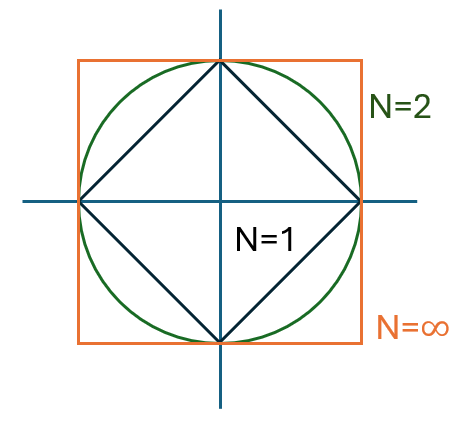
\includegraphics[width=0.5\textwidth]{assets/LN-Norm.png}
	\caption{Visualization of LN-Norm for all possible N values. lines represent unit distance from the origin under the chosen N-normalization.}
	\label{fig:LN-norm}
\end{figure}
Quality can be tuned directly or indirectly via configuration files in \texttt{compression\_configurations/\allowbreak quantization\_sweep/}.

\subsection{Entropy Coding}
The quantized channels are now transferred to the entropy coding method, where they are again broken up into blocks. If they are not \(\in \mathbb{N}^{b\times b}\), they again get padded with zeroes. They are then flattened to be \(z \in \mathbb{N}^{1\times b^2}\) 1D arrays using an algorithm called zigzag ordering, which utilizes following a previously initialized zigzag pattern, to rearrange the frequency values in such a way that bundles lower frequency values in the front as seen below.

\begin{figure}[H]
	\centering
	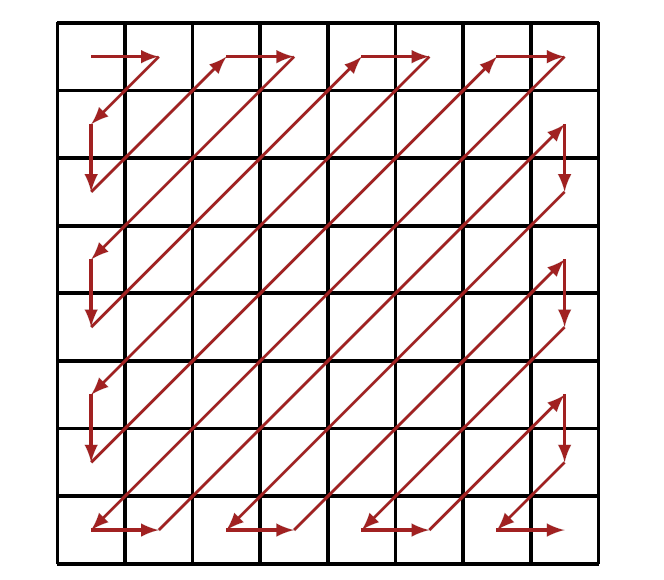
\includegraphics[width=0.8\linewidth]{assets/zigzag.png}
	\caption{Rearrangement of a \(8\times8\) block using zigzag pattern}
	\label{fig:zigzag}
\end{figure}

Then, as lower frequency values usually carry most information and energy, the so called DC component \(z_0 = F_Q(0,0)\) of each block is extracted and the difference is made with its predecessor from the block prior, in order to reduce the dynamic range of the DCT coefficients. This is called delta encoding, and the DC values are treated and even encoded differently from the remaining so called AC components. It is to be noted that luminance and chrominance values are separated here as elsewhere.

The AC components \(z_1,...,z_{b^2-1})\) are now forwarded to a method called run-length encoding, which for every value \(z_i \neq 0, i \in {1,...,b^2-1}\) returns a tuple as follows, given an array \(Z = [z_1, \ldots, z_{b^2-1}]\):

\begin{equation*}
	\mathcal{R}(Z) = \begin{cases}
		(z_i, c_i) & \text{for } a_i \neq 0 \text{ with } c_i \text{ preceding zeros} \\
		(0,0) & \text{if only zeroes remaining in the block}
	\end{cases}
\end{equation*}


\begin{algorithm}
	\caption{Run-Length Encoding Algorithm}
	\label{alg:jpeg-rle}
	\begin{algorithmic}[1]
		\Require $\text{zigzag\_array} = [z_1, \ldots, z_n]$
		\Ensure List of $(value, zero\_count)$ tuples with EOB marker
		
		\State $\text{encoded} \gets \emptyset$
		\State $\text{zero\_count} \gets 0$
		\For{each element $a_i \in \text{zigzag\_array}$}
		\If{$z_i = 0$}
		\State $\text{zero\_count} \gets \text{zero\_count} + 1$
		\Else
		\State $\text{encoded.append}((a_i, \text{zero\_count}))$
		\State $\text{zero\_count} \gets 0$ \Comment{Reset counter after non-zero value}
		\EndIf
		\EndFor
		\State $\text{encoded.append}((0, 0))$ \Comment{Add End-of-Block (EOB) marker}
		\State \Return $\text{encoded}$
	\end{algorithmic}
\end{algorithm}

Since the number of zeroes is concentrated in the end after the zigzag ordering, the returned array contains only a few tuples, which however are enough to describe the whole block. Since \(F_Q(b-1,b-1) = 0\) earlier, we do not need to worry about the \((0,0)\) EOB potentially elongating the block to be longer than its maximum size when decoding.


\subsubsection{Huffman Encoding}

\textbf{This Section Needs Citations}
Both the AC and the delta-encoded DC values of all blocks are finally forwarded, separated both by AC and DC as well as by luminance and chrominance, to the Huffman encoding algorithm. Here each symbol is counted and thus has its frequency determined. This frequency shall axiomatically serve as the probability of a symbol \(p(x_i)\) from now on.

Huffman encoding is a widely used lossless data compression algorithm that assigns variable-length codewords to symbols based on their probabilities. The key idea is to use shorter codes for more frequent symbols and longer codes for less frequent ones, minimizing the average codeword length. To further understand Huffman encoding, we first need some basic concepts from information theory. 
The information content\cite{sha48}\cite{Riley} of a symbol \( x_i \) with probability \( p(x_i) \) is defined as:
\[
I(x_i) = \log_2 \left( \frac{1}{p(x_i)} \right) = -\log_2 p(x_i).
\]
This measures how surprising or informative an event is: the less probable the symbol, the higher its information content.
The entropy \( H(X) \) of an information source is the expected (average) information content:
\[
H(X) = -\sum_{i=1}^{n} p(x_i) \log_2 p(x_i).
\]
Entropy represents the minimum average number of bits required to represent each symbol from the source.
From Shannon's Source Coding Theorem, the minimum expected codeword length \( L_{\text{min}} \) for a symbol \( x_i \) satisfies:
\[
H(X) \leq L_{\text{avg}} < H(X) + 1,
\]
where \( L_{\text{avg}} \) is the average length of the codewords. Huffman encoding achieves near-optimal compression, with \( L_{\text{avg}} \) very close to \( H(X) \).
Huffman encoding does this by constructing a prefix-free binary code (no codeword is a prefix of another) ensuring unambiguous decoding, using the following steps:
\begin{enumerate}
	\item \textbf{Frequency Calculation:} Compute the frequency (or probability) of each symbol in the input.
	\item \textbf{Priority Queue:} Build a min-heap where each node represents a symbol and its frequency.
	\item \textbf{Tree Construction:}  
	\begin{itemize}
		\item Repeatedly extract the two nodes with the smallest frequencies.
		\item Merge them into a new internal node with their combined frequency.
		\item Assign '0' to the left branch and '1' to the right branch.
		\item Reinsert the new node into the heap.
	\end{itemize}
	\item \textbf{Code Assignment:} Traverse the tree from the root to each leaf, recording the binary path to generate the Huffman code for each symbol.
\end{enumerate}

After the codewords were assigned for each group of values (Lum DC, Lum DC, Chrom DC, Chrom AC) and thus the so-called Huffman tables are created, the channels are iteratively encoded using the respective Huffman table, resulting in a long bitstream, which contains the data of the image. This alongside the Huffman tables themselves is forwarded to file encoding.

The benefit of using four different huffman tables instead of just one, is that the data often looks very different for each group, making it at least in most cases more efficient to use. However due to having multiple codewords for a recurring symbol, the header becomes larger.

Standard JPEG actually uses fixed Huffman tables instead, which is less compression efficient but definitely faster to encode.

Despite the fact that Huffman coding is quite optimal in terms of average word length, there are methods that provide even better compression such as arithmetic coding and asymmetric numeral systems (ANS). Arithmetic coding encodes data as a single fractional number, allowing symbols to occupy fractional bits and tightly approaching entropy limits. ANS improves on this by using integer-state transformations for similar compression gains while being computationally faster. Both methods excel where Huffman struggles, e.g. with highly skewed distributions (like 99 percent probable symbols), since they avoid Huffman's requirement of whole-bit codewords. Arithmetic coding is even used in JPEG XL, but due to patent issues in and around the 80s does not enjoy high popularity. For our project, we opted for Huffman coding, as it is not only easier, but because we believe that the focus of the work should lie on the lossy part of the compression and its impact on image classification. \cite{wiegand_source}
\subsection{File Encoding}
The file encoding method handles the final stage of our image compression pipeline, packaging all compressed components into a proprietary binary file format using our initials (.rde). The process begins by preparing the compression metadata - it converts the Huffman code tables and quantization matrices into JSON-serializable formats while preserving the original settings. The actual compressed bitstream (previously generated through Huffman encoding) gets processed into a byte-aligned format, with padding bits added if needed to complete the final byte.

The output file follows a specific structure: first a 4-byte header length indicator, followed by the JSON header containing all decompression parameters (quantization tables, Huffman dictionaries, image dimensions, and padding information), and finally the packed binary data representing the compressed image content. Alongside the binary file, the function generates comprehensive compression metrics including detailed size breakdowns (separating header overhead from actual image data), processing timings, and quality measurements like compression ratio and bits-per-pixel. These metrics get saved to a companion JSON file and can optionally be displayed in a formatted table, providing insights into the compression efficiency and the relative contributions of different components to the final file size. The implementation maintains careful byte-level control throughout the packaging process while handling all necessary data conversions between Python objects, JSON structures, and raw binary formats.
\subsection{Decompression Pipeline}
Decompression reverses all previous stages, while stripping the data of padded zeroes:
\begin{enumerate}
	\item \textbf{File Decoding}: Read binary data and extract header/metadata (quantization tables, Huffman codes, etc.) which are used in the later methods
	\item \textbf{Entropy Decoding}:
	\begin{itemize}
		\item \textbf{Huffman Decoding}: Reconstruct DC/AC coefficients
		\item \textbf{Run-Length Decoding}: Expand compressed AC coefficients
		\item \textbf{Delta Decoding}: Reverse DC coefficient differences
		\item \textbf{Inverse Zigzag}: Reshape 1D array to 2D frequency blocks
	\end{itemize}
	\item \textbf{Block Processing}:
	\begin{itemize}
		\item \textbf{Dequantization}: Multiply coefficients by quantization table values
		\item \textbf{IDCT}: Convert frequency-domain blocks to spatial pixels
	\end{itemize}
	\item \textbf{Chrominance Upsampling}: Upsample Cb/Cr channels if downsampled
	\item \textbf{Color Conversion}: Convert YCbCr back to RGB
	\item \textbf{Image Finalization}: Clamp pixel values, save image
\end{enumerate}
The decompression logic is implemented in \texttt{src/decompression.py}. It was in many cases quite challenging to get the correct output; especially block placement was a point of contention at first.

One point of interest here might be the handling of the upsampling. Before the colors can be converted back to RGB, the lower dimension chrominance channels need to be expanded accordingly. This can be done using any way of interpolation, we decided on nearest-neighbor for computation speed. However linear and other interpolation algorithms can be used to get better results.

\subsection{Evaluating Compression Distortion}

In order to evaluate compression distortion, two metrics are used: Structrual Similarity Index (SSIM) and PSNR (Peak Signal to Noise Ratio). These metrics are commonly used to compare "ground truth" images to processed images. \cite{wang2004image}\cite{psnr} The skimage package included as part of SciPy includes functions to calculate both SSIM and PSNR for a pair of images. These metrics are systematically evaluated across a sweep of images.

\subsection{Evaluation of Semantic Information}

While JPEG and other compression algorithms where designed largely with aesthetic quality preservation in mind, an important metric for modern compression algorithms is the preservation of semantic information. 
Evaluating the Semantic Preservation of a compression algorithm is essentially asking \enquote {Does the compressed image produce the same classification result with the same model input parameters?}. A competing requirement for compression performance is compression ratio, or the fraction of image data the compressed encoded image takes up. As the compression ratio approaches zero, it's expected that the semantic content of the image would be lost. Therefore, understanding what compression parameters improve compression rate without degrading semantic content is the subject of exploration for this next section.

We propose Confidence Error as a general summary metric for Semantic Preservation. Let $C_{err}$ represent our metric, the Confidence Error. Let $L_{max}$ be the highest probability label from and inference pass with ResNet50 on the uncompressed image. Let $P^{Lmax}_{uncompressed}$ be the probability of this label. Let $P^{Lmax}_{compressed}$ be the classification probability of label $L_{max}$ on the compressed image.

$$
\textrm{C}_{err} = \frac{\|P^{Lmax}_{uncompressed} - P^{Lmax}_{compressed}\|}{P^{Lmax}_{uncompressed}}
$$

When performing parameter sweeps across various compression parameters, we evaluate Confidence Error with the following algorithm
\begin{algorithm}
    \label{alg:Confidence Error Algorithm}
    \caption{Evaluating Confidence Error during compression parameter sweeps}
	\begin{algorithmic}[1]
    \Require{ Reference image $I_{ref}$, compressed image $I_{cmp}$, pretrained model $Res50$}
    \Ensure{ $C_{err}$ for the two images}
	\State $I_{ref, pp}$ = preprocess($I_{ref}$)
	\State $W_{ref \ outputs}$ = $Res50$.infer($I_{ref, pp}$)
	\State $P_{ref \ classes}$ = softmax($W_{outputs}$)
	\State $L_{max}$ = argmax({$P_{ref classes}$})
	\State $P^{Lmax}_{uncompressed}$ = $P_{classes}$[$L_{max}$]
	\State $I_{cmp, pp}$ = preprocess($I_{comp}$)
	\State $W_{comp \ outputs}$ = $Res50$.infer($I_{cmp, pp}$)
	\State $P_{cmp \ classes}$ = softmax($W_{outputs}$)
	\State $P^{Lmax}_{compressed}$ =  $P_{cmp \ classes}$[$L_{max}$]
	\State $\textbf{return}\ \frac{P^{Lmax}_{uncompressed} - P^{Lmax}_{compressed}}{P^{Lmax}_{uncompressed}}$
	\end{algorithmic}
\end{algorithm}

In this way, the semantic content is systematically compared and evaluated for each of the test images.

\subsubsection{Image Preprocessing for ResNet50}

ResNet50 requires images to be passed in cropped to a size of 224x224, and normalized to a pixel value range per channel of approximately -1 to 1. In order to avoid unfavorable crops of images, each image scalled down to a height of 256, and then center-cropped to 224x224 pixels. This way, a large portion of the center of the image is passed into the classifier. It is worth noting that this resize and crop preprocessing is essentially a lossy compression before the semantic information is extracted. If the only purpose of an compression algorithm is to extract semantic information, and the visual quality is of no concern, likely the most effective way to compress that image would be to downsample the image uniformally to the required size and perform a lossless encoding from there. There are many cases however, where the aesthetic quality of the image is important, and for these, the full image resolution is needed.

\subsection{Configuration Management}
\label{sec:config_management}
All compression parameters are stored in human-readable YAML files. These files are passed into the system via CLI (e.g., \texttt{results\_compression.py --config homemade\_compression\_jpeg\_like.yaml}).

Sweeps are conducted using \texttt{test/parameter\_sweeps.py}, which iterates over YAML directories for block sizes, downsampling levels, and quantization schemes.

Additional configuration directories (e.g., \texttt{quantization\_sweep\_chroma/}, \texttt{quantization\_sweep\_luma/}, \texttt{quantization\_sweep\_small\_blocks/}) were created during final testing to support more granular sweep control over chroma and luma quantization matrices.

\subsection{Implementation Highlights}

The repository is structured as follows:
\begin{itemize}
    \item \texttt{src/}: core pipeline (compression, decompression, utilities)
    \item \texttt{compression\_configurations/}: parameter sweep YAMLs
    \item \texttt{test/}: experimental evaluation, sweeps, classification
    \item \texttt{assets/}: test images
\end{itemize}

The test image suite was recently expanded and reorganized to support broader variation in content and file types. New naming conventions (e.g., \texttt{subject\_*}, \texttt{landscape\_*}) and formats (including TIFF, AVIF, PNG, and high-resolution RAW CR2) enable more granular benchmarking of compression behavior across diverse scenes, lighting conditions, and semantic content.

Key implementation goals included:
\begin{enumerate}
    \item Enabling experimentation with minimal code changes
    \item Supporting multiple image formats (PNG, JPG, AVIF, WEBP, CR2)
    \item Using only Python and standard packages (\texttt{numpy}, \texttt{PIL}, \texttt{scipy}, etc.)
    \item Support for advanced quantization experiments, including Quarter Gaussian and L-N norm-based matrices, with separate control over luminance and chrominance channels
\end{enumerate}

\subsection{Division of Work}
\label{sec:division-of-work}

While the initial division of work outlined in our February project proposal was tentative, the responsibilities naturally evolved during development. Although all team members collaborated conceptually, the division of work is outlined below:
\begin{itemize}
  \item George Roudebush: compression pipeline, parameter sweeps, quantization table and function development, baseline JPEG comparison, Semantic Preservation method development and testing, utility methods, test image dataset curation, and configuration integration, report results section, production of datasets for report and analysis of those datasets.
  \item Nicolas Drager: Entropy encoding, file coding, decompression pipeline, size estimation and compression metrics in file coding, bug fixes in all other compression methods, introducing raw image support, making it possible to switch between parameters, utility methods, huffman methods, testing methods, adapting the introduction in the report, implementation report up to \ref{sec:config_management}
  \item Muhammad Elarbi: decompression pipeline, padding error fixes, unit test development, raw image test dataset creation (CR2), output location handling, final-report drafting, documentation, and code cleanup
\end{itemize}